%!TEX root = Nanomat.tex
\ctitle{Struktur og morfologi på nanoskala}
\cstitle{Krystaller og nanokrystaller}
\paragraph{Andelen overflateatomer} Den viktigste forskjellen mellom nanomaterialer og makroskopiske materialer er andelen av atomene som befinner seg på overflaten. For makroskopiske materialer er andelen overflateatomer neglisjerbar, men når partiklenes størrelse reduseres til under ca. \SI{10}{\nano\meter} er andelen ikke lenger neglisjerbar. For overgangsmetaller kan denne andelen tilnærmes som en funksjon av nanopartikkelens radius,
\begin{equation}
	N_s/N_v \approx \frac{\SI{1}{\nano\meter}}{2R},
\end{equation}
men denne tilnærmingen bryter ned når man nærmer seg diametre på et par-tre nanometer.

\paragraph{Overflateenergi} Med den \emph{spesifikke overflateenergien} $\gamma$ til en gjenstand mener vi arbeidet som kreves for å øke overflatearealet til gjenstanden med én enhet. Sagt på differensialform:
\begin{equation}
	\label{eq:surface_work}
	\dW = \gamma \dA.
\end{equation}
Eller sagt på en annen måte:
\begin{equation}
	\label{eq:surface_work_alt}
	\gamma = \pdif{G}{A}{n,T,p}
\end{equation}

\paragraph{Overflateenergi på atomnivå} Økningen i overflateareal gjøres (konseptuelt) ved å flytte atomer fra volumet til overflaten av objektet. På mikroskopisk nivå er altså 
\begin{equation}
	\label{eq:gamma_microscopic}
	\gamma = \frac{1}{2}N_b\epsilon,
\end{equation}
der $N_b$ er tettheten av brudne bindinger (eller brudne bindinger pr. enhet overflate) og $\epsilon$ er bindingsenergien. Faktoren $1/2$ er med fordi bindingsenergien er assosiert med en binding, og en binding er mellom to atomer.

$N_b$ kan faktoriseres som $N_b=n_an_b$, der $n_a$ er tettheten av overflateatomer og $n_b$ er antall bindinger som blir brutt for hvert overflateatom. Da blir
\begin{equation}
	\label{eq:gamma_microscopic_expanded}
	\gamma = \frac{1}{2}n_an_b\epsilon.
\end{equation}

\paragraph{Kurvatur} Overflateenergien, og dermed det kjemiske potensialet, avhenger også av kurvaturen til overflaten. Dette kan forklares intuitivt som at en konkav overflate ``viser fram'' de reaktive atomene på overflaten, mens en konveks overflate ``gjemmer bort'' disse atomene. Endringen i kjemisk potensial som funksjon av kurvatur, er
\begin{equation}
	\Delta \mu = \mu_{\text{kurvet}} - \mu_{\text{flat}} = 2\gamma\frac{\Omega}{r}
\end{equation}
der $\mu_{\text{kurvet}}$ og $\mu_{\text{flat}}$ er kjemisk potensial for henholdsvis kurvet og flat overflate, $\Omega$ er volumet til et atom og $r$ er overflatens kurvaturradius. Kurvaturradien er positiv for konvekse overflater, negativ for konkave overflater, og uendelig for et plan.

\paragraph{Stress-tensor} Å flytte atomer til overflaten er ikke den eneste måten man kan øke overflatearealet på. Vi kan gjøre samme nytten ved å strekke objektet mens vi holder antallet overflateatomer konstant. I så fall vil $\dW$ avhenge av de krystallografiske aksene, og da må $\gamma$ erstattes med et element i en \emph{stress-tensor} $g_{ij}$, som tar hensyn til forskjell mellom retninger (der forskjellige retninger gir forskjellige $i$ og $j$, og dermed forskjellig $g_{ij}$). For en væske er $g_{ij}=\gamma$. Tensorer er stress, så det snakker vi ikke mer om nå.

\paragraph{Hvordan påvirkes gitterparameteren av størrelse?} 
%For en \emph{dråpe med væske} er $\dW$ gitt av forskjellen i trykk på innsiden og utsiden av dråpen, $\Delta P$:
%\begin{equation}
%	\dW = \Delta P \dV,
%\end{equation}
%slik at \eqref{eq:surface_work} blir til
%\begin{equation}
%	\Delta P \dV= \gamma \dA \implies \Delta P = \gamma \frac{\dA}{\dV}.
%\end{equation}
%I tilfellet med en kulerund dråpe er
%\begin{equation}
%	\frac{\dA}{\dV}=\frac{\dA}{\dRs}\frac{\dRs}{\dV} = \frac{\dA/\dRs}{\dV/\dRs}=\frac{\frac{\text{d}}{\dRs}4\pi R^2}{\frac{\text{d}}{\dRs} \frac{4}{3}\pi R^3}=\frac{2}{R}
%\end{equation}
%Hvis vi så ønsker å se på en \emph{sfærisk partikkel i fast fase} må $\gamma$ erstattes med stresstensoren. Dersom krystallstrukturen er kubisk, blir uttrykket for $g_{ij}$ greit nok:
%\begin{equation}
%	g_{ij}=g=\gamma+A\frac{\text{d}\gamma}{\dA}
%\end{equation}
La oss nå se på faste nanopartikler med en kubisk krystallstruktur. \emph{Kompressibiliteten} $\chi$ til et objekt er definert som
\begin{equation}
	\chi \equiv -\frac{\Delta V}{v\Delta P}
\end{equation}
der $v$ er volumet til en enhetscelle. Vi putter en minus foran slik at $\chi$ skal bli positiv, da $\Delta V$ ``alltid'' er negativ når $\Delta P$ er positiv. For kubiske krystaller er $v=a^3$, der $a$ er gitterparameteren. For kubiske krystaller har vi dermed
\begin{equation}
	\chi = -\frac{\Delta V}{a^3 \Delta P}.
\end{equation}
Hvis man bruker at $g_{ij}\dA=\dW=\Delta P \dV$\footnote{Dét, og svart magi.}, kan man utlede den relative endringen i gitterparameteren som funksjon av nanopartikkelens radius:
\begin{equation}
	\frac{\Delta a}{a} = -\frac{2}{3}\chi\frac{g_{ij}}{R}.
\end{equation}
Dette betyr at vi for små partikler får en \emph{sammentrekning} i gitteret, forårsaket av trykket innover mot partikkelen, som er proporsjonal med overflatespenningen, og invers proporsjonal med partikkelens størrelse. Dette er som regel sant for \emph{metaller}. I neste kapittel skal vi se at det er det \emph{motsatte} som er tilfelle for visse andre materialer - da \emph{utvider} gitteret seg når partiklenes størrelse minker.

%\paragraph{EXAFS og SEELFS} 

% \paragraph{Fonon} Fononer er ``kvasipartikler'' som representer atomenes vibrasjoner i gitteret. Fononer har lignende egenskaper som andre bølger/partikler, blant annet en frekvens. Når overflate/volum-forholdet til en partikkel øker, blir frekvensspekteret til fononene bredere. Bidraget til de lave frekvensene kommer fra overflateatomene, og bidraget til de høye frekvensene kommer fra økte interatomære krefter og dermed et mer rigid system. Dette får en effekt på smeltepunktet til nanopartikler, som vi kommer tilbake til i kapittelet om faseoverganger.

\cstitle{Nanopartiklers morfologi}

\paragraph{Polyedre} Nanopartikler vil i enkelte tilfeller være formet som enkle polyedere. Hva de forskjellige polyedrene som det refereres til i teksten, ser ut som, kan man enkelt finne ut med et internett-bildesøk. For ordens skyld er noen av de vanligste polyedrene vist i Figur~\ref{fig:polyhedra}. 

Et \idx{avstumpet polyeder} er det man får når man tar med seg et polyeder til tresløyden og pusser ned alle hjørnene med sandpapir, slik at man får en ny fasett med like mange kanter som det var kanter som møttes i hjørnet man pusset ned\footnote{Bréchnigac refererer til tider til et generelt avstumpet oktaeder som ``cubo-octahedra'', men dette stemmer ikke. Et kubooktaeder er grensetilfellet man får når man pusser ned oktaederet så mye at de opprinnelige kantene i oktaederet har null lengde.}.
\begin{figure}[H]
	\bmd\centering
	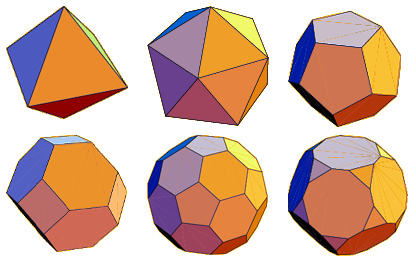
\includegraphics[width=\linewidth]{polyhedra3.png}
	\caption{Vanlige polyedre. Øvre rad, fra venstre: oktaeder, ikosaeder, dodekaeder. Nedre rad, fra venstre: avstumpet oktaeder, avstumpet ikosaeder, avstumpet dodekaeder.}
	\label{fig:polyhedra}
\emd\end{figure}
Merk at de forskjellige sidekantene ofte har forskjellige lengder, og dermed noe forskjellig form, fra de som er vist i Figur~\ref{fig:polyhedra}.

\paragraph{Likevektsformen til en makroskopisk krystall} Formen til en krystall avhenger av betingelsene når krystallen vokser, og disse betingelsene er ofte langt unna termodynamisk likevekt. Men ved likevektsbetingelser vil krystallen innta én bestemt form, nemlig formen som minimerer den totale overflateenergien. For en væske er dette en kule, men for en krystall kan overflateenergien være forskjellig avhengig av orienteringen til krystallflaten. Derfor må man minimere summen av bidrag fra hver av fasettene, nemlig
\begin{equation}
	E_s = \sum_i \gamma_iA_i,
\end{equation}
der $\gamma_i$ er overflateenergien og $A_i$ er overflaten til fasett $i$. En viss George Yuri Victorovich Wulff\footnote{Takk for fullt navn på herr G Wulff, Gaute!} viste at man får til dette hvis formen er et polyeder der avstanden $h_i$ fra sentrum av krystallen til fasett $i$ er proporsjonal med overflateenergien $\gamma_i$ for alle $i$. \emph{Wulffs teorem} er altså at
\begin{equation}
	\frac{\gamma_i}{h_i} \text{ er konstant}
\end{equation}
når krystallen har sin likevektsform. 

\paragraph{Wulff-konstruksjon} Wullfs teorem gir oss umiddelbart en metode for å konstruere likevektsformen til en krystall når vi vet hvordan overflatespenningen avhenger av krystallens orientering. Se side 9-10 i Bréchnigac et. al. Noen resultater av en slik konstruksjon er:
\begin{itemize}
	\item Metaller med fcc-struktur danner et avstumpet oktaeder der $(111)$-planet og $(100)$-planet vises.
	\item Metaller med bcc-struktur danner et dodekaeder.
	\item Enkle ioniske krystaller som \ce{NaCl} og \ce{MgO} danner en kube. Alle ioniske krystaller har høy grad av anisotropi når det kommer til overflateenergi, så overflaten vil kun bestå av én familie med krystallplan.
\end{itemize}
% ENVELOPE!

\paragraph{Likevektsformen til nanopartikler} Wulffs teorem gjelder for makroskopiske krystaller. Vi har gode modeller for de interatomære kreftene i de fleste metaller, så gjennom numeriske simuleringer kan vi sjekke om Wullfs teorem også holder når partiklene blir veldig små. Det gjør det ikke: gjennom slike molekylsimuleringer har det vist seg at fcc-metaller danner fire forskjellige former: avstumpet oktaeder, kuboktaeder, ikosaeder og avstumpet dodekaeder. Hvilken form en partikkel har, avhenger av størrelsen på partikkelen:
\begin{itemize}
	\item For veldig små partikler er den mest stabile formen et ikosaeder, fordi denne formen er nærmest sfærisk og kun viser $(111)$-fasetter, som har lav overflatespenning. Denne formen kan ikke partikkelen beholde når den blir større, både fordi den ikke har kubisk symmetri, og fordi atomene i midten av ikosaederet blir veldig komprimert.
	\item Innenfor et visst størrelsesområde er likevektsformen et avstumpet dodekaeder.
	\item Forbi en viss størrelse danner partikkelen et avstumpet oktaeder (som har kubisk symmetri, og dermed kan danne en fcc-struktur internt). Denne overgangen fra ikke-krystallinsk til krystallinsk struktur kan variere voldsomt fra metall til metall: den skjer ved 200 atomer for gull og ved 30000 atomer for kobber.
\end{itemize}

\paragraph{Kvasismelting} Når partiklene er små, er ikke forskjellen mellom de forskjellige formene så veldig stor i forhold til den tilfeldige, termiske energien i omgivelsene. I praksis vil man derfor observere at partikler antar mange forskjellige former. Særlig når størrelsen er ca. ved overgangen, vil partiklene oscillere eller fluktuere kaotisk mellom forskjellige former - dette fenomenet kalles \idx{kvasismelting}.

\paragraph{Kanteffekter} Atomene som befinner seg på kantene mellom de forskjellige fasettene har enda flere løse bindinger enn atomene inni fasettene på overflaten, og de får dermed høyere overflateenergi. Dette er fordi de har en høy positiv kurvatur, i motsetning til flater eller avrundede kanter. Dette gjør kanter og hjørner mer løselige enn resten av materialet. I praksis fører dette til at gjenstander som løses opp, gradvis blir avrundet.\footnote{Litt som steiner på stranden.} % En formel som beskriver dette kvantitativt er
%\begin{equation}
%\label{eq:curv_temp}
%	\frac{C_{\text{kurvet del av materialet}}}{C_{\text{flat del av materialet}}}=\exp{\frac{\gamma\Omega}{k_BT}\left(\frac{1}{r_1}+\frac{1}{r_2}\right)}
%\end{equation}
%der $C$ er løseligheter og $r$ er kurvaturradier (jeg aner ikke hvorfor det er to av dem). Legg merke til at andelen kurvet materiale minker eksponensielt med temperaturen, men ikke gidd å huske på selve uttrykket.

\cstitle{Morfologi for partikler med støtte}
\paragraph{Wulff-Kaichew-teoremet} La oss så se på partikler som er støttet til et substrat. I Figur~\ref{fig:surface_support} mener man med avstumpingen $\Delta h_s$ hvor dypt partikkelen hadde trengt inn i substratet dersom den hadde hatt formen den ville hatt som fri partikkel.
\begin{figure}[H]
	\bmd\centering
	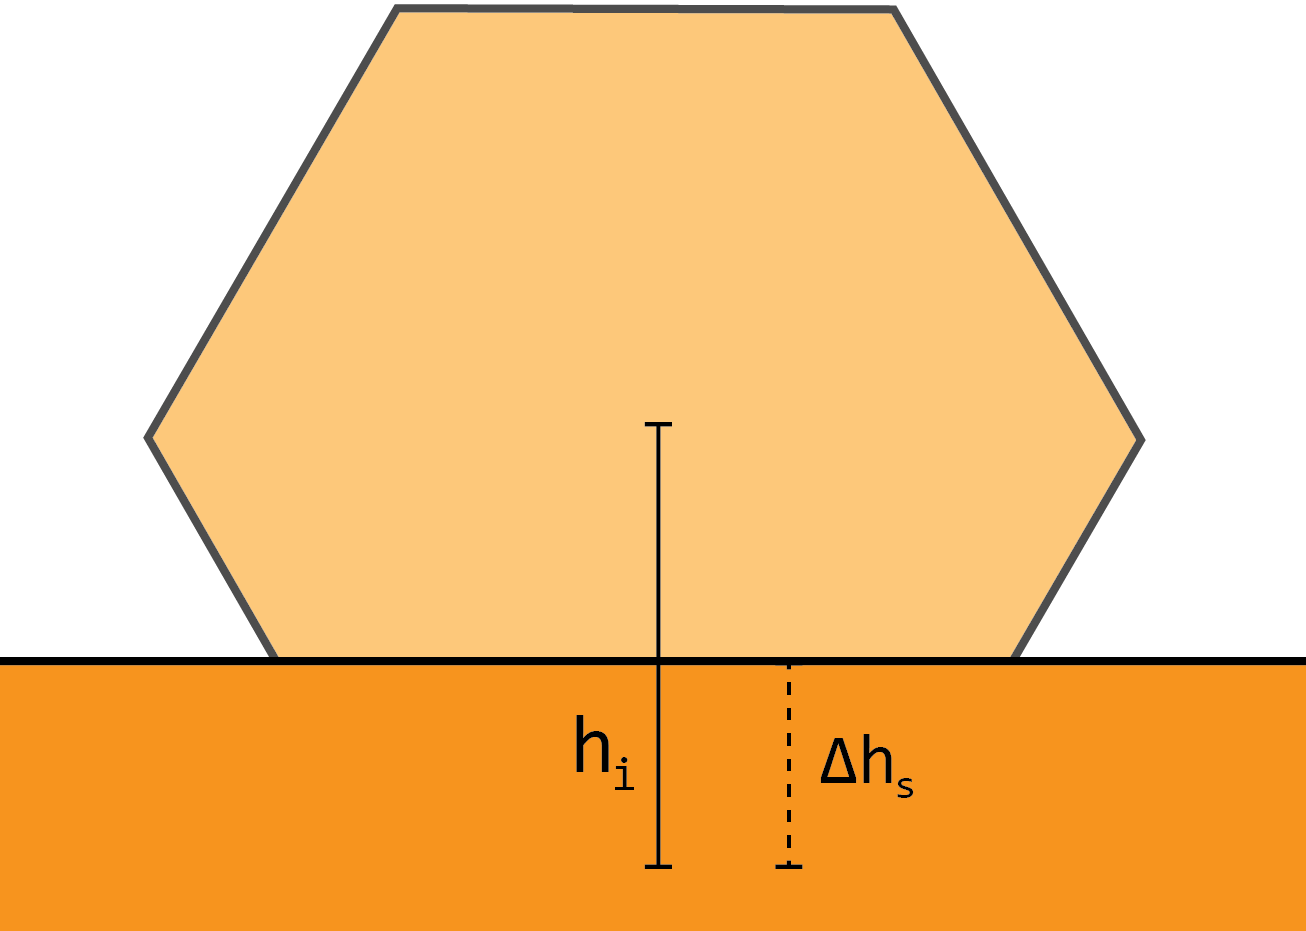
\includegraphics[width=\linewidth]{surface-01.png}
	\caption{Skisse av en nanopartikkel (med heksagonalt tverrsnitt) som er støttet til et substrat.}
	\label{fig:surface_support}
\emd\end{figure}
Avstumpingen $\Delta h_s$ er gitt ved Wulff-Kaichew-relasjonen
\begin{equation}
	\label{Wulff-Kaichew}
	\frac{\Delta h_s}{h_i} = \frac{E_{\text{adhesjon}}}{\gamma_i}.
\end{equation}
Her er adhesjonsenergien $E_{\text{adhesjon}}$ energien per enhet overflate som kreves for å løsne fra hverandre to krystaller (én av substratmaterialet, én av partikkelmaterialet) som opprinnelig er i kontakt. Denne energien kan være alt fra $0$ (dette er tilfelle hvis partiklene overhodet ikke interagerer med overflaten) til $2\gamma_i$. Hvis den er større enn 2$\gamma_i$, dannes det ikke partikler, men en kontinuerlig film på overflaten.

\paragraph{Effekter på grunn av grenseflatespenning} Wulff-Kaichew-teoremet antar at partikkelen og substratet har akkurat samme krystallstruktur, med samme gitterparameter. I så tilfelle vil partikkelens form være uavhengig av størrelse. Dette er sjelden tilfellet; i stedet vil partikkelen, siden den har en viss elastisitet, forvrenges for å tilpasse seg krystallstrukturen til substratet. Dette fører til at det oppstår en \emph{grenseflatespenning}. Etter hvert som partikkelen vokser, vil den uungåelig passere et punkt der det er mer gunstig å danne dislokasjoner enn det er å fortsette å strekke på krystallstrukturen for å tilpasse seg substratet. Når dette skjer, vil partikkelen ``falle sammen'' litt, og spre seg utover på bekostning av høyde. Etter hvert som partikkelen fortsetter å vokse, vil det dannes flere dislokasjoner, slik at høyden til partikkelen oscillerer rundt en viss verdi.
\vfill
\cstitle{Avbildningsmetoder}
Dette har jo ikke all verden å gjøre med resten av kapittelet, men la oss til slutt snakke litt om metoder vi kan bruke for å se på disse nanopartiklene.

\paragraph{Elektronmikroskopi} TEM (transmisjons-elektron\-mikroskopi) utføres ved å sende elektroner gjennom prøven. Elektronstrålen går videre gjennom en rekke (elektron)linser før den treffer en skjerm. Prøvene må nødvendigvis være svært tynne, og slike prøver kan være vanskelige å preparere.

\paragraph{Scanning-probe-mikroskopi} STM (scanning tunneling microscopy) og AFM (atomic force microscopy) er noen av mikroskopimetodene som gir høyest oppløsning (subatomær presisjon). Disse er basert på at en probe med en atomært tynn spiss føres ned mot prøven og følger profilen til prøven, og enten registrerer kvantemekanisk tunneleringsstrøm (i STM, og dette fungerer kun på ledende prøver) eller interatomære krefter mellom spissen og prøven (i AFM, og dette fungerer for alle prøver). Dette gjør det mulig å få 3D-bilder av prøven med ekstremt høy presisjon i høyderetning (bedre enn \SI{0.1}{\nano\meter}).

\paragraph{Konvolusjonseffekt i AFM-avbilding} I lengderetningen sliter man med at resultatene påvirkes av formen til spissen, på en slik måte at bildet viser rundere kanter og større partikler enn det som faktisk er tilfelle. Dette kalles en konvolusjonseffekt og har ingenting med matematisk konvolusjon å gjøre. Hvis man kjenner formen på spissen kan man korrigere for dette i etterkant og vise en riktigere størrelse på partiklene, men man mister likevel informasjon om den vertikale profilen, og hvor på substratet partikkelen begynner.

\paragraph{GISAXS} står for \emph{Grazing Incidence Small Angle X-Ray Scattering}. Røntgenstråler sendes nesten parallellt med overflaten til substratet, og ``sneier'' borti partikler og klynger av atomer som er støttet til substratet. Ved å analysere hvordan partiklene sprer røntgenstrålen, kan man måle egenskaper som gjennomsnittlig høyde og størrelse på partiklene, og gjennomsnittlig avstand mellom to partikler.
